\documentclass{beamer}
\usepackage[utf8]{inputenc}
\usepackage{graphicx}
\usepackage{xcolor}
\usepackage{listings}


\title{TIL-Script Typechecker}
\author{Filip Peterek}
\institute{VSB -- Technical University of Ostrava}
\date{June 2022}

\begin{document}

\frame{\titlepage}

\section{Project goals}

\begin{frame}
    \frametitle{Project goals}
    \begin{itemize}
        \item Create a working typechecker for TIL constructions
        \item Plot typechecking graph to an image
        \item Write extensible code to allow further development
    \end{itemize}
\end{frame}

\section{Accomplished goals}

\begin{frame}
    \frametitle{Accomplished goals}
    \begin{itemize}
        \item Working typechecker
        \item Graph plotting
        \item TIL-Script parser
        \item Context recognition
    \end{itemize}
\end{frame}

\section{Implementation}

\begin{frame}
    \frametitle{Implementation}
    \begin{itemize}
        \item Kotlin
        \item Gradle
        \item Antlr
    \end{itemize}
\end{frame}

\begin{frame}
    \frametitle{Parser Implementation}
    \begin{itemize}
        \item Existing TIL-Script grammar has been utilized
            \begin{itemize}
                \item Slight tweaks were necessary to make it work with Antlr
            \end{itemize}
        \item Parser is generated using Antlr
        \item Resulting AST is converted to a custom structure
    \end{itemize}
\end{frame}

\begin{frame}
    \frametitle{Typechecker Implementation}
    \begin{itemize}
        \item For typechecking to succeed, all names must be defined
        \item This is ensured in a separate step
        \item If at least one undefined name is found, processing ends
        \item Errors are printed to stdout
    \end{itemize}
\end{frame}

\begin{frame}
    \frametitle{Typechecker Implementation}
    \begin{itemize}
        \item Recursive implementation
        \item Aliases are expanded, expansions are compared
        \item Double execution is ignored
        \item Trivializations force construction of independent scopes
        \item Type deduction is unsupported
        \item Errors are, yet again, printed to stdout
    \end{itemize}
\end{frame}

\begin{frame}
    \frametitle{Context Recognition}
    \begin{itemize}
        \item Context recognition is also supported
        \item Recursive implementation
        \item No errors can be detected at this point
    \end{itemize}
\end{frame}

\begin{frame}
    \frametitle{Program Output}
    \begin{itemize}
        \item Errors are printed to stdout
        \item Script information is written to a JSON file
            \begin{itemize}
                \item Constructions
                \item All subconstructions of said constructions
                \item Definitions
                \item Constructed type
                \item Type of TIL-Script statement
                \item Context
            \end{itemize}
        \item Typechecking graph is created as an SVG image
    \end{itemize}
\end{frame}

\begin{frame}
    \frametitle{Graph Plotting}
    \begin{itemize}
        \item No third party libraries
        \item Indentation is necessary due to lengths of type ids
        \item Monospace font
    \end{itemize}
\end{frame}

\begin{frame}
    \frametitle{Graph Plotting}
    \begin{center}
        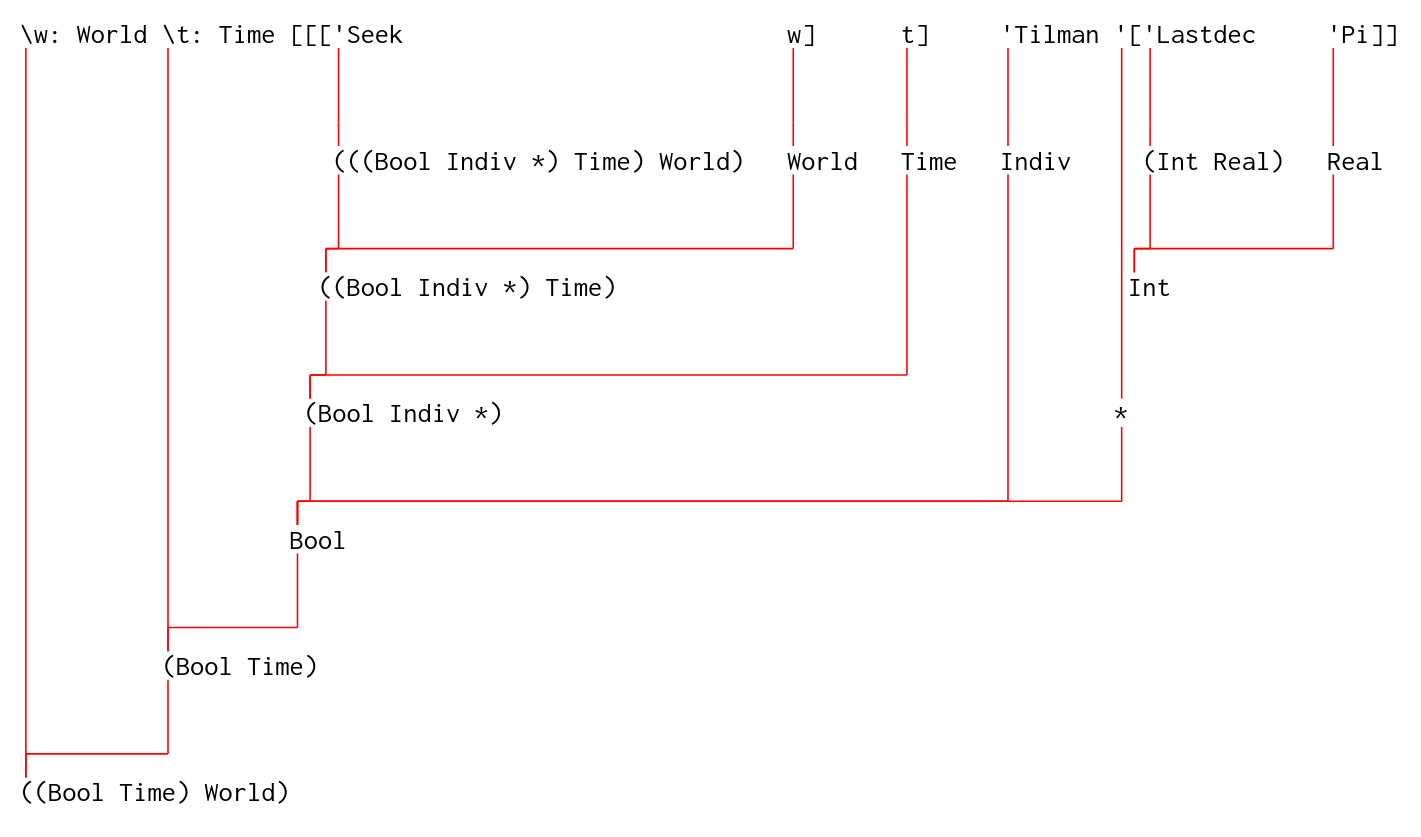
\includegraphics[width=0.9\columnwidth]{graph.png}
    \end{center}
\end{frame}

\section{Future Work}

\begin{frame}
    \frametitle{Possible Improvements}
    \begin{itemize}
        \item LSP
            \begin{itemize}
                \item Text editor integration
                \item Code completion
                \item Error reporting
                \item Refactoring
                \item Supported by all major editors (Vim, Emacs)
            \end{itemize}
    \end{itemize}
\end{frame}

\begin{frame}
    \frametitle{Possible Improvements}
    \begin{itemize}
        \item Interactive browser application
            \begin{itemize}
                \item Web application available online
                \item Allows online text editing
                \item Provides on-the-fly syntax and type coherence checking
                \item Opportunity to utilize graphs
            \end{itemize}
    \end{itemize}
\end{frame}

\begin{frame}
    \begin{center}
        \Huge The End
    \end{center}
\end{frame}

\end{document}
